
\section{ProFaaStinate}
\label{sec:profaastinate}
% Das hier kann dann weg richtig?

The next section provides an overview of the ProFaaStinate paper proposed by Schirmer et al. \cite{schirmer2023profaastinate}. First, it digs into the real-world problems it aims to tackle, breaks down its key concepts, and also points out some problems we have identified. Subsequently, this section delves into the detailed explanation and implementation of its components. Finally, we will offer insights into how to effortlessly extend the implementation with custom schedulers and other supplementary components. Additionally, we outline the conventions developers must uphold to ensure adherence to a seamless workflow.
\begin{figure}
    \centering
    \includegraphics[width=.9\linewidth]{figures/profaastinate/architecture_gray.pdf}
    \caption{ProFaaStinate improves conventional FaaS platforms with a priority queue and Call Scheduler. Asynchronous calls are placed into the priority queue, managed by the Call Scheduler. The scheduler operates in two states, responding to monitoring data: busy mode prioritizes urgent calls, while idle mode handles both urgent and non-urgent calls. \cite{schirmer2023profaastinate}}
    \label{fig:og-profaastinate}
\end{figure}

\subsection{Concept}
\label{sec:ProFaaStinate_Concept}
 
Serverless Function-as-a-Service (FaaS) platforms encounter significant challenges due to the volatility in the number of requests they need to handle. The number often increases in peak hours compared to periods with low-loads, such as nighttime.

This issue is particularly leveraged in self-hosted environments, where resources are limited and increased by the absence of dynamic scaling mechanisms. Hence, users may need to scale their systems to defend themselves against peak loads, ensuring urgent tasks are executed immediately. However, this scaling results in underutilized resources during periods of low request load, leading to an imbalance between the potential of the system and its actual load. This imbalance decreases the overall cost efficiency.

In response to these challenges, ProFaaStinate introduces an approach where it differentiates between synchronous (urgent) and asynchronous (non-urgent) function calls. Synchronous function calls need to be executed immediately, which is helpful in scenarios where the calling component awaits the response. In contrast, asynchronous function invocations are tagged with a deadline, indicating the latest time by which the function must be executed. This critical distinction, as mentioned by Schirmer et al. \cite{schirmer2023profaastinate}, is currently not taken into consideration in serverless platforms like Nuclio. In such environments, both types of calls are treated the same and are executed immediately upon invocation.

ProFaaStinate addresses this limitation by expanding Function as a Service (FaaS) platforms, allowing them to delay the execution of asynchronous calls based on scheduling strategies, shown in Figure \ref{fig:og-profaastinate}. This is done by enabling the redirection of asynchronous function invocations. Synchronous calls are processed the same as in the default implementation, they are immediately executed when they arrive at the call Api by the Call Executor. Asynchronous calls, on the other hand, are placed in a priority queue with a specific latency target after they arrive. Lastly, a Call Scheduler then consumes this queue and executes the calls by calling the Call Executor, allowing the system to delay function calls \cite{schirmer2023profaastinate}.

The Scheduler can operate in two different states, the idle state, and the busy state. In the busy state, it will only process urgent calls, which are calls where the deadline falls within a specified threshold. This allows the system to decrease its resource consumption. In the idle state, it can additionally process calls where the deadline exceeded the threshold, meaning that their deadline is further in the future. The system can switch the state based on specified conditions. Hence, it can decrease its carbon impact or reduce the cost of the system \cite{schirmer2023profaastinate}.


\subsection{Problem Statement}
Considering the original ProFaaStinate concept and implementation, this section proposes the motivation for our new implementation. \cite{schirmer2023profaastinate}

First of all, it is important to know that there is currently no abstraction layer separating the Nuclio platform from ProFaaStinate. This integration is deeply embedded in the Call Api. In order to improve the maintainability of the system and facilitate future development, it is necessary to separate the code according to the principle of separation of concerns. In ProFaaStinate's flow (Figure \ref{fig:og-profaastinate}) a synchronous call, consequently gets enqueued as a entry in the priority queue. However, this task is non-trivial, because the logic to transform and enqueue requests have to be performed inside the call Api. 

In the initial implementation of ProFaaStinate, they used a PostgreSQL\footnote{\url{https://www.postgresql.org/}} database to implement the priority queue. However, this is not ideal when operating it as a time-sensitive queue, due to the fact that it is not indexed and therefore not sorted. It adds additional overhead in terms of enhanced orchestration, maintenance, and configuration. A dedicated PostgreSQL instance also entails increased resource utilization. The database also relies on the network to insert and receive entries, which potentially leads to latency and bandwidth-related bottlenecks.

% requires increased resource usage vs higher resource utilization - ist das nicht irgendwie das gleiche???
These challenges become more relevant in distributed environments, where the decision between centralized or decentralized approaches becomes critical. Opting for a centralized approach results in higher resource utilization and broader bandwidth and latency limitations. On the other side, the decentralized approach requires increased resource usage and orchestration effort.

Lastly, ProFaaStinate only provides a single scheduler, which is controlled by its state (busy and idle). However, this approach limits developers to the use of the provided scheduler. This scheduler only allows increasing or decreasing the number of concurrent requests based on the state. Hence the implementation of advanced strategies, such as executing specific requests based on metrics, is restricted. Furthermore, integrating multiple schedulers entails a challenge, because there is only one controllable state for the scheduler, which limits the expandability of the system. \cite{schirmer2023profaastinate}
%%%%%%%

\subsection{Requirements}
\label{sec:requirements}

% Überleitungsatz
Having understood the problems of the current system, we now turn to the requirements by deriving the minimum functional requirements from the current capabilities. The non-functional ones result from the fact that they are intended to prevent the current problems. Recording the requirements is necessary in order to be able to better measure which tasks have been fulfilled and which have not.

\subsubsection{Functional Requirements}
\label{sec:functional-req}
The following functional requirements define what our product must do and what its features are.
\begin{itemize}
    \item \textbf{Asynchronous function execution}: The platform should be extended so that delayed function executions are possible; these should be stored in a kind of queue. Deferrable functions are characterized by an associated deadline that determines the latest possible execution. 

     \item \textbf{Different Scheduler Types}: The system must implement multiple scheduler types for executing asynchronous functions. Each scheduler should serve distinct purposes, providing flexibility beyond simple idle and busy states. Additionally, the system must ensure that all job deadlines are met.

    \item \textbf{Configuration Flexibility}: Users should have the ability to adjust various parameters and settings during runtime to tailor the system to their specific research needs. This includes options such as adjusting resource allocations or modifying scheduler behavior on-the-fly.
    
\end{itemize}

\subsection {Non-functional requirements}
\label{sec:non-functional-req}
The several non-functional requirements, that are the general properties or quality attributes of a system, were taken into account during the development of the system. 
\begin{itemize}
    \item \textbf{Abstraction Layer}: To improve system organization, a layer is implemented that separates the Nuclio platform and ProFaaStinate, allowing for easier component changes without system-wide impact.
    \item \textbf{Modular extensible architecture}: Creation of a modular architecture that allows new components such as a scheduler to be written quickly without having to think deeply about the interaction of other components. 
    \item \textbf{Documentation}: Comprehensive documentation should be provided to help users understand the software and its architecture.
    \item \textbf{Unit Tests} are essential to ensure the robustness and reliability of the software. The project manager did not directly specify a specific test coverage rate, so we opted for the industry standard of 75\%\footnote{\url{https://www.atlassian.com/continuous-delivery/software-testing/code-coverage}}.
\end{itemize}


\begin{figure*}
    \centering
    \includegraphics[width=0.98\linewidth]{figures/profaastinate/ProFaaStinate.pdf} 
    \caption{ProFaaStinate's implementation is integrated within Nuclio, where it immediately executes synchronous functions. Asynchronous functions are forwarded to ProFaaStinates Nexus for subsequent processing and delayed execution.}
    \label{fig:MPGA-architecture}
\end{figure*}

\subsection{Implementation Overview}
As in the original implementation, we also implemented ProFaaStinate inside Nuclio \cite{schirmer2023profaastinate}. Our implementation consists of three core components, which are depicted in figure \ref{fig:MPGA-architecture}, it includes the Nexus, the Nexus Queue and the Schedulers, each of them is responsible for individual tasks. It also includes several supporting components that are required to complement the core implementation. Just like in the original approach, we have seamlessly integrated our components into Nuclio. The Components are housed inside the dashboard container described in section \ref{sec:nuclio}. Our implementation intercepts incoming function invocation requests inside the dashboard RESTServer, without making changes to the rest of the Nuclio's processing flow. When a function is invoked with default headers, its execution follows Nuclio's standard flow without delay. A request is identified as asynchronous, if it includes a deadline header specifying the time in milliseconds until the function must be executed, it is then forwarded to ProFaaStinate's Nexus. The Nexus abstracts the incoming function invocations and pushes them into the Nexus Queue. The schedulers operate concurrently as Goroutines. These employ different strategies to retrieve items and forward synchronous requests to the dashboard so that Nuclio executes the functions.

\subsection{Components}

The following section provides an overview of the implemented components. This includes the supportive components, including the Environment Registry, the Load Balancer and the Elastic Deployer. It will also propose the core components, including the Nexus, the Nexus Queue, and the Scheduler. For the last mention we will also provide a small guide on how a developer can build and integrate their own scheduler. 

\subsubsection{Environment Registry}
\label{sec:env-registry}
The environment service serves as a central register for managing environment variables within the Nexus system. It reads essential variables that do not change during runtime and initializes itself by setting default values if required. This distinguishes it from the Variable of the REST Api which may be changed during runtime. 

Currently, the following environment variables are available: DEPLOY\_ENVIRONMENT, which specifies whether Nuclio is running in a Docker or Kubernetes environment, and NUCTL\_NAMESPACE, indicating the namespace of the Nuclio function container. 

By centralizing the management of environment variables, the registry improves the stability and consistency of the system.

\subsubsection{Load Balancer}
\label{sec:load-balancer}
The Load Balancer has the task of efficiently distributing the workload across the various time frames in the Nexus system and represents the counterpart to the Busy and IDLE state of the underlying paper\cite{schirmer2023profaastinate}.

It is responsible for determining the maximum number of parallel requests executed at the same sliding window. The scheduler communicate with the Load Balancer and tell them when they invoke a function synchronously. After the end of a sliding window, the Load Balancer then calculates the system load and tries to optimize the number maximum parallel requests per second with the target load for cpu and memory. A time window is used here to prevent the system from throttling too much and consuming large amounts of CPU with a high frequency of calculations. The slidingWindowsDuration is set to 5 seconds by default, while the target load for CPU and memory are set to 0.6.
This system was modeled after the autopod scaler of kubernetes, which also scales linearly with the formular\footnote{\url{https://kubernetes.io/docs/tasks/run-application/horizontal-pod-autoscale/}}:
{\small
\[
\text{desiredReplicas} = \lceil \dfrac{\text{currentReplicas} \times \text{currentMetricValue}}{\text{desiredMetricValue}}\rceil
\]
}

Since we primarily want to create load balancing with our system, we have only considered memory and cpu usage as metrics in the Load Balancer. If both metrics are now set, by default at 60\%, the system calculates the following formulas
{\small
\[
\text{desiredNumberMem} = \frac{\text{executedFunctionCalls} \times \text{targetLoadMem}}{\text{usedLoadMem}}
\]

\[
\text{desiredNumberCPU} = \frac{\text{executedFunctionCalls} \times \text{targetLoadCPU}}{\text{usedLoadCPU}}
\]

\[
\text{parllelRequests} = \left\lceil \frac{\text{desiredNumberMem} + \text{desiredNumberCPU}}{2} \right\rceil
\]
}


The user can dynamically adjust the Load Balancer by interacting with the PUT REST endpoint "/load-balancer". The parameters for configuration include:

\begin{itemize}
\item targetLoadCPU: A value between 0.0 and 1.0 specifying the desired CPU load.
\item targetLoadMemory: A value between 0.0 and 1.0 specifying the desired memory load.
\item maxParallelRequests: This parameter, when set, disables the dynamic behavior of the Load Balancer and instead sets a fixed maximum number of parallel requests.
\end{itemize}

\begin{figure}
    \centering
    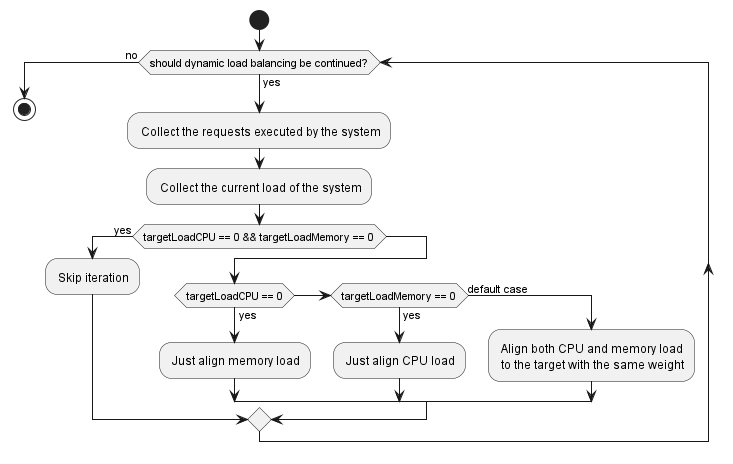
\includegraphics[width=\linewidth]{figures/profaastinate/load-balancer-schedule.png}
    \caption{These parameters allow adaptive fine-tuning of the Load Balancer's behavior to meet specific performance and resource utilization requirements. The following activity diagram illustrates the logic sequences within the Load Balancer, whereby the direct setting of maxParallelRequests leads to the termination of the while condition, so that the calculation is no longer dynamic.}
    \label{fig:og-profaastinate}
\end{figure}

%%% Beispiel ja oder nein? Folgendes von GPT
In order to better understand this, we assume a scenario with the parameters:
\begin{itemize}
    \item Number of executed function calls: 100
    \item Target load for CPU: 0.7
    \item Target load for memory: 0.6
    \item Used load for CPU: 0.8
    \item Used load for memory: 0.5
\end{itemize}

Using the provided formulas:
\[
\text{{desiredNumberMem}} = \dfrac{100 \times 0.6}{0.5} = 120
\]
\[
\text{{desiredNumberCPU}} = \dfrac{100 \times 0.7}{0.8} = 87.5
\]
\[
\text{{maxParallelRequests}} = \lceil \frac{120 + 87.5}{2} \rceil = \lceil 103.75 \rceil = 104
\]

In this example, the Load Balancer would be configured to allow a maximum of 104 parallel requests to maintain optimal performance considering both CPU and memory usage.

\subsubsection{Elastic Deployer}
\label{sec:elastic-deploy}
In general, the deployer is used to save resources in the deployment by automatically stopping function containers that have not been used for a certain time window, which is set to 1 minute by default. It saves all containers associated with Nuclio and how long they are still running.
To stop certain containers, it forwards stop requests to the dedicated deployer services for Docker or Kubernetes, which do this for it. The environment services are integrated through an abstract layer via an interface, so that new environments could easily be deployed using the same approach, which is consistent with our desire for a modular extensible architecture.
It also constantly communicates with the various schedulers to ensure that the required containers are running when they need to be called synchronously. It can also continue functions that have already been stopped via the interface.

It is important to note that while a Docker implementation was successfully implemented, the Kubernetes implementation could not be completed within the given timeframe as it became too complex. This component was an attempt to imitate the Premium feature of Nuclio. Various ideas were collected and implemented for this, but in the end, the components created was not sufficiently convincing in terms of performance, and the deployer was deactivated for the final evaluation. 

\subsubsection{Nexus}
\label{sec:nexus}
The Nexus, as its name suggests, serves as the central hub of our implementation. It is responsible for the connection between various components. Moreover, it initializes all other components, which include the schedulers and the necessary supportive components. Supportive components are components that provide data to schedulers, which are necessary for their strategy. One of those supportive components is the Load Balancer. The Nexus also manages the Nexus Queue and provides it to all components that need them. During its initialization, the Nexus starts the schedulers and supportive components. Additionally, it exposes a RESTful endpoint to dynamically start, stop, or configure schedulers and other supportive components during runtime. When the Nexus receives an asynchronous request, it extracts the deadline subsequently from it. Then, it transforms the request into a Nexus Queue entry, the entry consists of a function invocation and the extracted deadline, which is needed to index the entry.

\subsubsection{Nexus Queue}
\label{sec:nexus-queue}
The Nexus Queue integrates the delay logic, which is responsible for storing the function invocation entries until subsequent processing. We used the deadline to index the entries, meaning the first entire of the queue has the lowest deadline, and vice versa. Therefore we employed a Go Heap, which is a self-balanced tree structure and fits perfectly for the indexed entries. We opted for this approach over the initial implementation with PostgreSQL, due to its lightweight and sorted nature. In addition, it provides some performance benefits because the entries are stored within the memory. One drawback of this approach in contrast to the original implementation with PostgreSQL, is the missing data resilience. The entries are lost in case of a system failure.

We tried to keep the implementation of the Nexus Queue as straightforward as possible, due to its crucial role in being easily expansible in the future. Our design ensures and feasible integration of custom methods for specific use cases, allowing necessary enhancements to the queue. This flexibility enables the system to evolve.

\subsubsection{Base Scheduler}
\label{sec:base-scheduler}

In our implementation, we refactored the approach of a single scheduler to view it more as a group of independent components, rather than a single entity, enhancing their expandability. This approach aligns with the composite design pattern, popular in Go, allowing us to structure the schedulers as composite objects composed of smaller, individual components. Each scheduler shares a common core concept: extracting items from the Nexus queue based on specific conditions while considering external factors and then transforming these items into synchronous requests to Nuclio's dashboard for immediate execution. These schedulers operate at regular intervals, with the timeout duration between intervals adjustable alongside other custom parameters in the configuration.

When building custom schedulers, some conventions must be taken into consideration. The scheduler has to be initialized inside the Nexus and integrated within the list of known schedulers so that the Nexus can start it. The Nexus Queue must be passed to the scheduler during initialization. Furthermore, it needs methods to start, stop, and gather the status of the scheduler. A developer might use the existing schedulers as orientation. The Nexus will then use those methods to start and stop the scheduler upon initialization. The strategy of the scheduler is recommended to be implemented within its executeScheduler method. There are no limitations to that, but developers have to take care that the schedulers won't interfere with each other.


\subsection{Scheduler Types}
\label{sec:scheduler-types}
In the following section, we will provide detailed explanations of the various scheduler types implemented in our system. Our implementation proposes three different scheduler types, which are designed to target independent goals: The Deadline Scheduler, Idle Scheduler, and Bulk Scheduler.

Firstly, we will explain the Deadline Scheduler, which is responsible for meeting the deadlines of function invocations. Then, we will provide information for the Idle and Bulk schedulers, those schedulers are designed to minimize the impact on resources. Specifically, the Deadline Scheduler targets the reduction of cold starts. All of the implemented schedulers communicate with the Load Balancer.

To speed up development and improve the configurability of the system, we have also integrated support for starting and stopping all schedulers via the REST Api. Using the endpoints "/scheduler/{schedulername}/start" and "/scheduler/{schedulername}/stop", researchers can quickly start or stop the scheduler's operations as needed. This implementation speeds up the development process considerably and thus meets the non-functional requirement for configuration flexibility.

    \begin{figure}
        \centering
        \includegraphics[width=.9\linewidth]{figures/profaastinate/deadline_scheduler_example.pdf}
        \caption{An instance of the Deadline Scheduler. Assuming that the deadlines for $Entry_1$ and $Entry_2$ in the queue are below a specified threshold, the Deadline Scheduler removes these entries ($Entry_1$ and $Entry_2$) from the queue for processing. This involves executing synchronous function invocation requests for these entries.}
        \label{fig:deadline-scheduler-example}
    \end{figure}
    \subsubsection{Deadline Scheduler} 
\label{sec:deadline-scheduler}
The deadline scheduler ensures that every function invocation in the queue is processed before its deadline. This process is depicted in Figure \ref{fig:deadline-scheduler-example}. This is done by periodically checking the entry at the front of the queue, which is always the function invocation with the lowest deadline in the Nexus Queue. If the deadline of this task falls within a configured threshold, the scheduler executes the function invocation. This execution includes the removal of the entry from the queue and subsequent synchronous requests to Nuclio's Dashboard.

This process, of checking, removing, and finally sending a synchronous request, is done as long as the deadline of the first entry in the queue falls within the configured threshold. If there are no items left in the queue, meaning the deadline for the first items is later than the threshold, the scheduler pauses for a specified timeframe. In contrast to the other schedulers, it is not restricted by the Load Balancer. It can make as many parallel requests as needed to process every task falling within the deadline. However, the scheduler also registers its requests in the Load Balancer, meaning that it claims a slot in the Load Balancer for a parallel request before removal of the entry, and releases the slot after sending the request. It can allocate more slots than available, to fulfil its objective to process all entries before their deadline. This can lead to the potential blocking of other schedulers.



    \begin{figure}
        \centering
        \includegraphics[width=.9\linewidth]{figures/profaastinate/idle_scheduler_example.pdf}
        \caption{An instance of the Idle Scheduler. With a maximum parallel request constraint set to 3 by the Load Balancer, this scheduler operates independently of specific time frame deadlines for queued items. Instead, it systematically removes the first three entries from the queue and processes requests for each entry ($Entry_1$, $Entry_2$, and $Entry_3$), adhering to the maximum parallel request limit enforced by the Load Balancer.}
        \label{fig:idle-scheduler-example}
    \end{figure}
    \subsubsection{Idle Scheduler}
\label{sec:idle-scheduler}
The Idle Scheduler has a significant dependence on the Load Balancer because the Load Balancer constrains its functionality. It operates similarly to the Deadline Scheduler by running at periodic intervals. It also extracts the first entry from the queue. However, unlike the Deadline Scheduler, the deadline of the item does not need to fall within a configured deadline threshold. The Idle Scheduler can process as many concurrent tasks as allowed by the Load Balancer. The Idle Scheduler will only process new entries if there are free slots available. In contrast to the Deadline Scheduler, it cannot allocate more slots than the maximum parallel requests set by the Load Balancer. Additionally, it processes the first entries of the queue, meaning the invocations with the lowest deadline, similar to the Deadline Scheduler, due to the sorted nature of the queue. This process is illustrated in Figure \ref{fig:idle-scheduler-example}.


    \subsubsection{Bulk Scheduler} 
\label{sec:bulk-scheduler}

    \begin{figure}
        \centering
        \includegraphics[width=.9\linewidth]{figures/profaastinate/bulk_scheduler_example.pdf}
        \caption{An instance of the Bulk Scheduler. This scheduler operates by identifying the largest group of entries with the same function invocation, where the associated function worker is paused. It ensures that this group of entries does not surpass the maximum parallel request limit. Subsequently, the scheduler removes this group of entries and processes them accordingly ($Entry_1$, $Entry_3$, and $Entry_5$).}
        \label{fig:bulk-scheduler-example}
    \end{figure}

The third and final scheduler we implemented is the Bulk scheduler, which tries to reduce cold start times. These occur when a function worker is paused and started again for processing incoming function invocations. In the context of Kubernetes, this means that the replicas of the function workers are scaled to zero, consequently, no function workers are currently running for that function. Nuclio utilizes this idea by scaling unused function workers to zero. Nuclio only starts a function worker again if a function for the worker is invoked. Nuclio uses this concept to minimize the resource footprint of function workers which are not frequently requested.

However, a challenge arises using Nuclio because paused function workers might be periodically called in intervals where the function scales down before it is invoked again. Consequently, the container starts up every time the function is invoked. Those start-ups entail resource usage and increase the latency. The Bulk Scheduler is designed to address this issue. The concept behind this scheduler is to batch requests for paused containers. It aggregates function invocations for the same function and sends them in direct succession, thereby ensuring only one cold start for the initial function invocation. The subsequent invocations can use the already unpaused container. Therefore, the scheduler identifies the most entries in the Nexus Queue that invoke the same function, which is currently paused or scaled to zero, and invokes them, as depicted in Figure \ref{fig:bulk-scheduler-example}. This process is also done in periodic intervals. The Bulk Scheduler depends on the number of max parallel requests ensuring the system runs below its resource utilization target.
